\documentclass{beamer}

\usepackage{multicol}
\usepackage{multimedia}
\usepackage{mathtools}

\newcommand{\Poincare}{Poincar\'{e}}
\newcommand{\Complex}{\mathbb{C}}
\newcommand{\Real}{\mathbb{R}}
\newcommand{\Rational}{\mathbb{Q}}
\newcommand{\Integer}{\mathbb{Z}}
\newcommand{\Natural}{\mathbb{N}}

\usetheme[progressbar=title]{metropolis}           % Use metropolis theme
\title{The Millennium Prize Problems}
\subtitle{A PGR Seminar in Two Parts}
\date{}
\author{Luke Smallman}
\institute{Cardiff University} \titlegraphic{\hfill
\includegraphics[height=1.5cm]{logo}}


\begin{document}
  \maketitle
  \begin{frame}{Structure}
      \begin{multicols}{2}
          \tableofcontents
      \end{multicols}
  \end{frame}

  \section{Introduction}
  \begin{frame}{Introduction}
      \begin{itemize}
          \item The Millennium Prize Problems were seven unsolved problems
              set out by the Clay Mathematics Institute
      \pause
          \item The Millenium Prize Problems are now six unsolved problems
              and one solved problem.
      \pause
          \item They have a certain level of infamy due to the Clay
              Mathematics Institute's promise of \$1 million for a correct
              proof of any of the problems
      \end{itemize}
  \end{frame}
  \begin{frame}{Even Elementary knows what the MPP are}
      \begin{center}
      \movie[width=\textwidth]{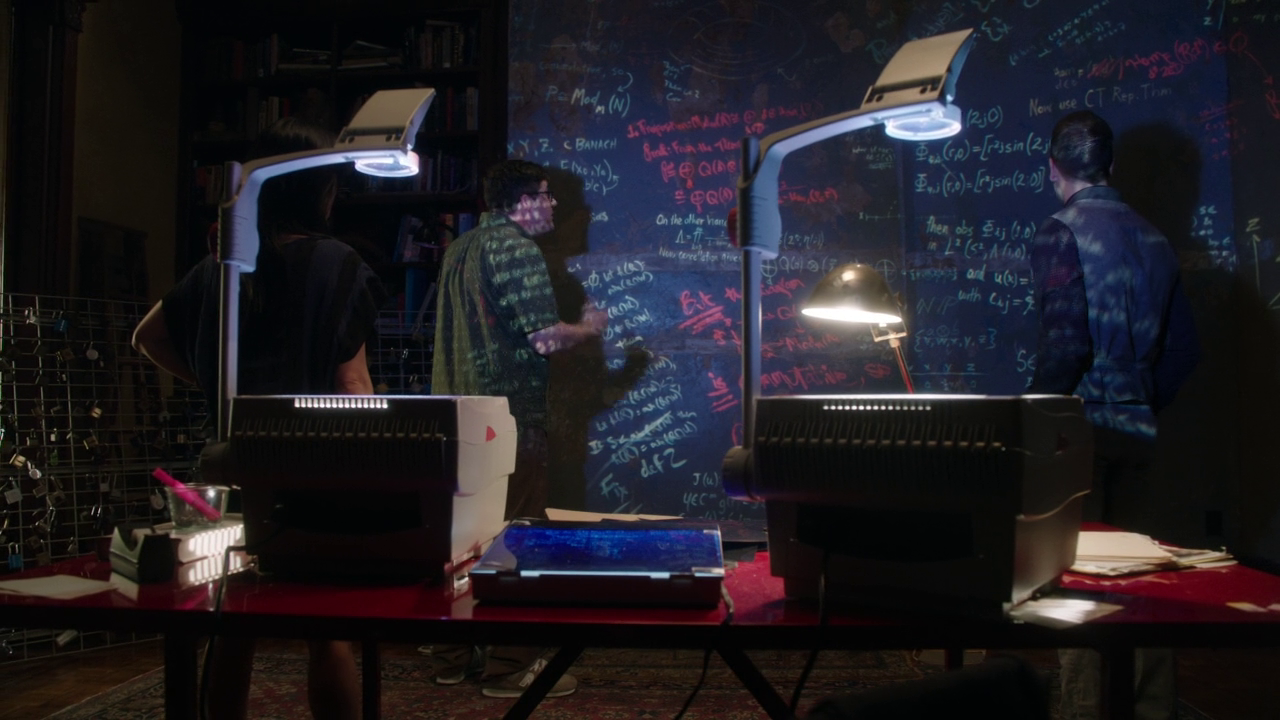
\includegraphics[width=\textwidth]{PvNPscreen.png}}{PvNP.mkv}
  \end{center}
  \end{frame}

  \section{P versus NP}
  \begin{frame}{P vs NP}
      \begin{block}{Problem Statement}
          Prove or disprove that $\mathcal{P} = \mathcal{NP}$
      \end{block}
  \end{frame}

  \section{Hodge Conjecture}
  \begin{frame}{Hodge Conjecture}
      \begin{block}{Problem Statement}
          Prove that on a projective non-singular algebraic variety over
          $\Complex$, any Hodge class is a rational linear combination of
          classes $cl(Z)$ of algebraic cycles.
      \end{block}
  \end{frame}

  \section{Riemann Hypothesis}
  \begin{frame}{Riemann Hypothesis}
      \begin{block}{Problem Statement}
          Prove that all non-trivial zeros of $\zeta(s)$ have real part
          $\frac{1}{2}$
      \end{block}
  \end{frame}

  \section{Yang-Mills Existence and Mass Gap}
  \begin{frame}{Yang-Mills Existence and Mass Gap}
      \begin{block}{Problem Statement}
          Prove that for any compact simple gauge group $G$, a non-trivial
          quantum Yang-Mills theory exists on $\Real^4$ and has a mass gap
          $\Delta > 0$.
      \end{block}
  \end{frame}

  \section{Navier-Stokes Existence and Smoothness}
  \begin{frame}{Navier-Stokes Existence and Smoothness}
      \begin{block}{Problem Statement}
          Prove that there exist smooth solutions with finite energy of the
          Navier-Stokes equations for any given divergence-free initial
          velocity field with no external force applied on either $\Real^3$
          or $\Real^3/\Integer$, OR prove that there exists a divergence-free
          intial velocity field and a smooth external force which does not
          have a smooth solution with finite energy.
      \end{block}
  \end{frame}

  \section{Birch and Swinnerton-Dyer Conjecture}
  \begin{frame}{Birch and Swinnerton-Dyer Conjecture}
      \begin{block}{Problem Statement}
          Prove that the Taylor expansion at $s=1$ of the incomplete
          $L$-function $L(C, s)$ of non-singular projective model $C$ of a
          curve $C_0$ defined by $f(x, y) = 0$ for a polynomial
          $f \in \Rational [x, y]$ has the form
          $c(s-1)^r + \text{higher order terms}$ with
          $r = \mathrm{rank}(C(\Rational))$.
      \end{block}
  \end{frame}

  \section{\Poincare{} Conjecture}
  \begin{frame}{\Poincare{} Conjecture}
      \begin{block}{Problem Statement}
          Prove that every simply connected, closed 3-manifold is
          homeomorphic to the 3-sphere.
      \end{block}
  \end{frame}


\end{document}
